%!TEX root = ../../../main.tex

\subsection{MICAGes dataset}
    There does not exist a dataset dedicated to the evaluation of robustness of hand gesture recognition w.r.t. viewpoint changes. Therefore, in our work, we carefully design a dataset collected from multiple viewpoints in indoor environment with complex background. Our dataset consists of nine dynamic hand gestures which correspond to controlling commands of electronic home appliances. Each gesture is a combination of hand movement following a pre-defined direction and changing of hand shape in a natural manner.

    Five Kinect sensors {K1, K2, K3, K4, K5} are setup at five positions in a square simulation room of $16m^2$ (Fig. \ref{Fig:MICAGes1}). This work aims to capture hand gestures under multiple viewpoints synchronously. The subjects are invited to stand at a fixed position approximately 2 meters in front of the center view. The Kinect sensors provide both RGB and Depth data captured at frame rate of 20 fps and resolution of 640 $\times$ 480, which allows us to capture a multi-view and multi-modal dataset.
    \begin{figure}[h]
        \centering
        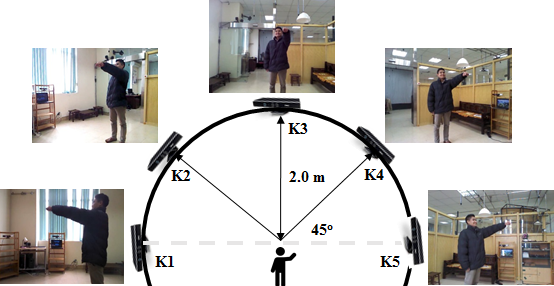
\includegraphics[width=0.8\linewidth]{figs/MICAGes1.png}
        \caption{Environment setup to capture MICAGes dataset.}
        %\vspace{-0.3cm}
        \label{Fig:MICAGes1}
    \end{figure}

    \begin{figure}[htbp]
        \centering
        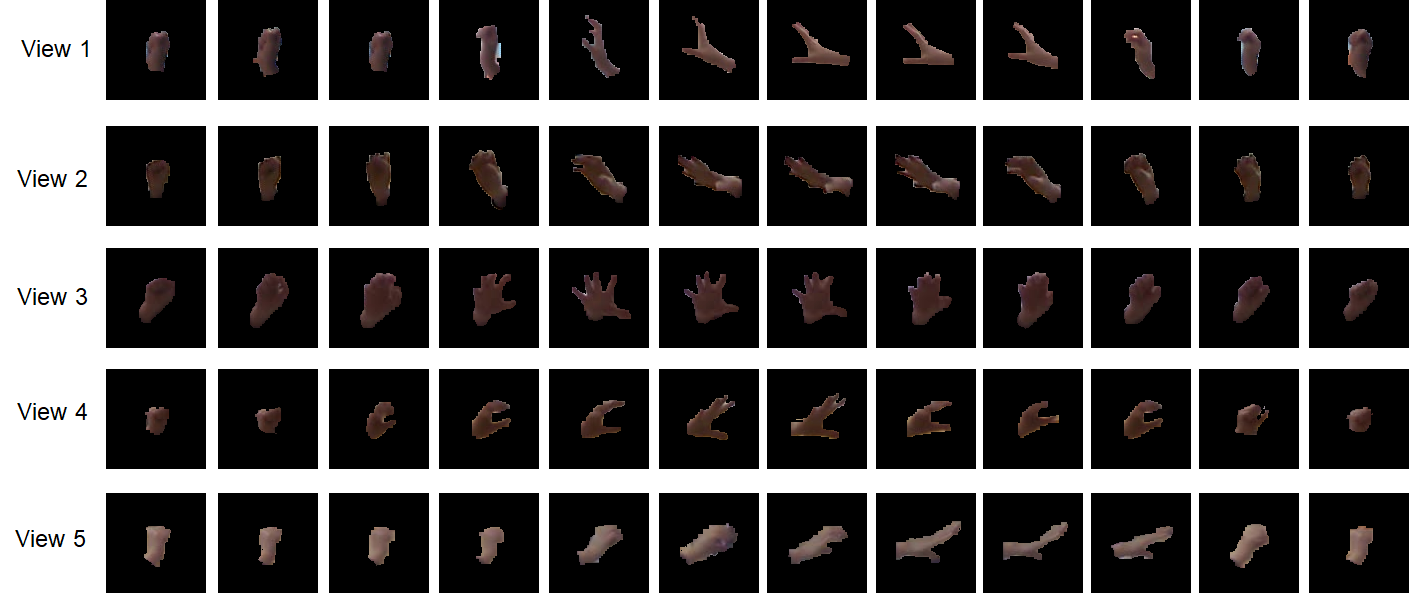
\includegraphics[width=0.9\linewidth]{figs/MICAGes2.png}
        \caption{Illustration of a gesture belonging to the $6^{th}$ class observed from five different views.}
        %\vspace{-0.3cm}
        \label{Fig:MICAGes2}
    \end{figure}
    Twelve participants (08 males and 04 females) are voluntary to perform gestures one after another, each gesture three times. Totally, the dataset contains 1620 (5 views $\times$ 09 gestures $\times$ 12 subjects $\times$ 3 times) dynamic hand gestures.
